\documentclass[a4paper,10pt]{scrartcl}

\usepackage{polski}
\usepackage[utf8]{inputenc}
\usepackage{graphicx}
\usepackage{enumerate}
\usepackage{pdflscape}

\title{Laboratorium 8}
\author{Filip Malinowski}
\date{\today}

\pdfinfo{%
  /Title    (Laboratorium 8)
  /Author   (Filip Malinowski)
}

\begin{document}

\title{Sprawozdanie z laboratorium 8}
\author{Filip Malinowski}
\date{\today}

\maketitle

Do programu zostały dodane drzewo binarne oraz
drzewo czerwono-czarne.
Drzewo czerwono-czarne zostało poprawione.
\\

Teoretyczna złożność dodawania elementu do
drzewa binarnego wynosi
\begin{math}
  log(n).
\end{math}
Według pomiarów do 1000 elementów złożoność
wynosi
\begin{math}
\frac{1}{10} * n
\end{math}
, zaś dla 10 000 elementów i wzwyż wynosi
\begin{math}
 n * 10^x
\end{math}
z x równym 0, zwiększającym się o 1 co każde
10 razy więcej elementów.
\\

Złożoność obliczeniowa odczytu w binarnym
drzewie poszukiwań powinna wynosić
\begin{math}
 n*log(n)
\end{math}
przez ilość elementów w drzewie równą
\begin{math}
n
\end{math}
, oraz złożoność dostępu równą
\begin{math}
 log(n)
\end{math}.
Według pomiarów złożność odczytu wynosi
\begin{math}
 log(n)
\end{math}
do 1000 elementów, natomiast od 1000 wzwyż
wynosi
\begin{math}
 log(n) * n
\end{math}.
\\

Złożoność obliczeniowa dodawania elementów do
drzewa czerwono-czarnego powinna wynosić
\begin{math}
  log(n).
\end{math}
Według pomiarów złożoność dodawania wynosi
\begin{math}
\frac{1}{10} * n
\end{math}.
\\

Złożoność obliczeniowa odczytu w drzewie
czerwono-czarnym powinna wynosić
\begin{math}
 n*log(n).
\end{math}
Również przez to, że ilość elementów
w drzewie to
\begin{math}
 n
\end{math}
, a czas dostępu wynosi
\begin{math}
 log(n)
\end{math}.
Według pomiarów złożność odczytu wynosi
\begin{math}
 log(n)
\end{math}
do 1000 elementów, natomiast od 1000 wzwyż
wynosi
\begin{math}
 log(n) * n
\end{math}.
\\

Gorszy od drzewa RB czas dodawania elementów do 
drzewa binarnego wynika z braku optymalizacji
głębokości drzewa tak jak to się dzieje
w drzewie RB. Trzeba wykonywać więcej porównań
elementów i przebywać większą drogę z racji
większej głębokości drzewa.

Odczyt elementów z obu drzew jest porównywalny
ponieważ działa na takiej samej zasadzie: drzewo
jest przeglądane w głąb i zwracane są jego
wszystkie elementy.


\pagebreak

\begin{landscape}
\begin{figure}
 \centering
 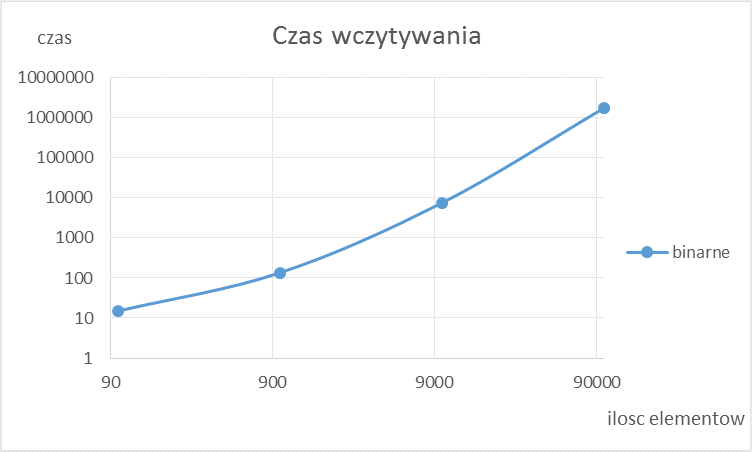
\includegraphics{wczytywanie}
 \caption{Wykres złożoności obliczeniowej wczytywania}
\end{figure}

\begin{figure}
 \centering
 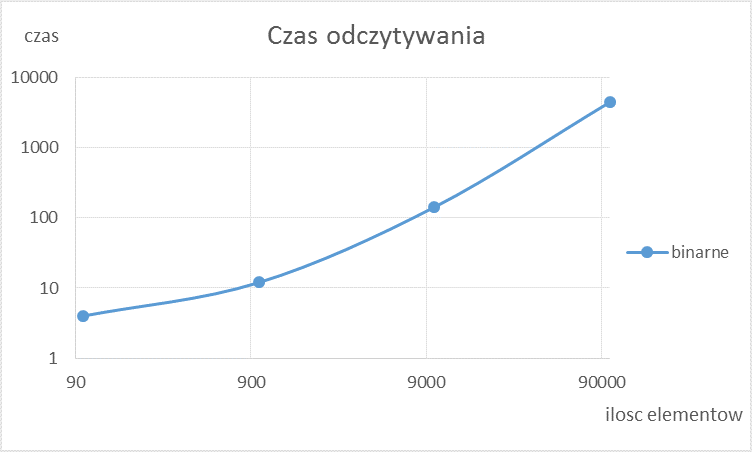
\includegraphics{odczytywanie}
 \caption{Wykres złożoności obliczeniowej odczytywania}
\end{figure}

\end{landscape}


\end{document}